\chapter{循环神经网络}\label{chap:Rnn}

\begin{introduction}
	\item 语言模型~\ref{Rnn:1}
	\item 循环神经网络是啥~\ref{Rnn:2}
	\item 基本循环神经网络~\ref{Rnn:3}
	\item 双向循环神经网络~\ref{Rnn:4}
	\item 深度循环神经网络~\ref{Rnn:5}
	\item 循环神经网络的训练~\ref{Rnn:6}
	\item 训练算法:BPTT~\ref{Rnn:7}
	\item 梯度爆炸和消失问题~\ref{Rnn:8}
	\item RNN的应用:语言模型~\ref{Rnn:9}
	\item 向量化~\ref{Rnn:10}
	\item Softmax层~\ref{Rnn:11}
	\item 语言模型的训练~\ref{Rnn:12}
	\item 交叉熵误差~\ref{Rnn:13}
	\item 编程实战:RNN的实现~\ref{Rnn:14}
\end{introduction}


在前面的文章系列文章中,我们介绍了全连接神经网络和卷积神经网络,以及它们的训练和使用。他们都只能单独的取处理一个个的输入,前一个输入和后一个输入是完全没有关系的。但是,某些任务需要能够更好的处理\textbf{序列}的信息,即前面的输入和后面的输入是有关系的。比如,当我们在理解一句话意思时,孤立的理解这句话的每个词是不够的,我们需要处理这些词连接起来的整个\textbf{序列};当我们处理视频的时候,我们也不能只单独的去分析每一帧,而要分析这些帧连接起来的整个\textbf{序列}。这时,就需要用到深度学习领域中另一类非常重要神经网络:\textbf{循环神经网络(Recurrent Neural Network)}。RNN种类很多,也比较绕脑子。不过读者不用担心,本文将一如既往的对复杂的东西剥茧抽丝,帮助您理解RNNs以及它的训练算法,并动手实现一个\textbf{循环神经网络}。


\section{语言模型}\label{Rnn:1}


RNN是在\textbf{自然语言处理}领域中最先被用起来的,比如,RNN可以为\textbf{语言模型}来建模。那么,什么是语言模型呢?

我们可以和电脑玩一个游戏,我们写出一个句子前面的一些词,然后,让电脑帮我们写下接下来的一个词。比如下面这句:
\begin{lstlisting}[numbers=none]
    我昨天上学迟到了,老师批评了 _ _ _ _。
\end{lstlisting}

我们给电脑展示了这句话前面这些词,然后,让电脑写下接下来的一个词。在这个例子中,接下来的这个词最有可能是『我』,而不太可能是『小明』,甚至是『吃饭』。

\textbf{语言模型}就是这样的东西:给定一个一句话前面的部分,预测接下来最有可能的一个词是什么。

\textbf{语言模型}是对一种语言的特征进行建模,它有很多很多用处。比如在语音转文本(STT)的应用中,声学模型输出的结果,往往是若干个可能的候选词,这时候就需要\textbf{语言模型}来从这些候选词中选择一个最可能的。当然,它同样也可以用在图像到文本的识别中(OCR)。

使用RNN之前,语言模型主要是采用N-Gram。N可以是一个自然数,比如2或者3。它的含义是,假设一个词出现的概率只与前面N个词相关。我们以2-Gram为例。首先,对前面的一句话进行切词:
\begin{lstlisting}[numbers=none]
    我 昨天 上学 迟到 了 ,老师 批评 了 _ _ _ _。
\end{lstlisting}


如果用2-Gram进行建模,那么电脑在预测的时候,只会看到前面的『了』,然后,电脑会在语料库中,搜索『了』后面最可能的一个词。不管最后电脑选的是不是『我』,我们都知道这个模型是不靠谱的,因为『了』前面说了那么一大堆实际上是没有用到的。如果是3-Gram模型呢,会搜索『批评了』后面最可能的词,感觉上比2-Gram靠谱了不少,但还是远远不够的。因为这句话最关键的信息『我』,远在9个词之前!

现在读者可能会想,可以提升继续提升N的值呀,比如4-Gram、5-Gram.......。实际上,这个想法是没有实用性的。因为我们想处理任意长度的句子,N设为多少都不合适;另外,模型的大小和N的关系是指数级的,4-Gram模型就会占用海量的存储空间。

所以,该轮到RNN出场了,RNN理论上可以往前看(往后看)任意多个词。

\section{循环神经网络是啥}\label{Rnn:2}

循环神经网络种类繁多,我们先从最简单的基本循环神经网络开始吧。

\subsection{基本循环神经网络}\label{Rnn:3}

图\ref{fig:Rnn1}是一个简单的循环神经网络如,它由输入层、一个隐藏层和一个输出层组成:

\begin{figure}[!h]
	\centering
	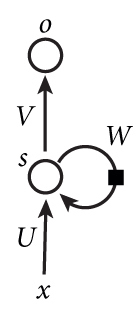
\includegraphics[width=0.15\textwidth]{Rnn1.jpg}
	\caption{简单的循环神经网络}
	\label{fig:Rnn1}
\end{figure}

纳尼?!相信第一次看到这个玩意的读者内心和我一样是崩溃的。因为\textbf{循环神经网络}实在是太难画出来了,网上所有大神们都不得不用了这种抽象艺术手法。不过,静下心来仔细看看的话,其实也是很好理解的。如果把上面有W的那个带箭头的圈去掉,它就变成了最普通的\textbf{全连接神经网络}。$x$是一个向量,它表示\textbf{输入层}的值(这里面没有画出来表示神经元节点的圆圈);$s$是一个向量,它表示\textbf{隐藏层}的值(这里隐藏层面画了一个节点,你也可以想象这一层其实是多个节点,节点数与向量$s$的维度相同);$U$是输入层到隐藏层的\textbf{权重矩阵}(读者可以回到第\ref{chap:Bp}章神经网络和反向传播算法,看看我们是怎样用矩阵来表示\textbf{全连接神经网络}的计算的);$o$也是一个向量,它表示\textbf{输出层}的值;$V$是隐藏层到输出层的\textbf{权重矩阵}。那么,现在我们来看看$W$是什么。\textbf{循环神经网络}的\textbf{隐藏层}的值$s$不仅仅取决于当前这次的输入$x$,还取决于上一次\textbf{隐藏层}的值$s$。\textbf{权重矩阵}
$W$就是\textbf{隐藏层}上一次的值作为这一次的输入的权重。

如果我们把上面的图展开,\textbf{循环神经网络}也可以画成图\ref{fig:Rnn2}这个样子:

\begin{figure}[!h]
	\centering
	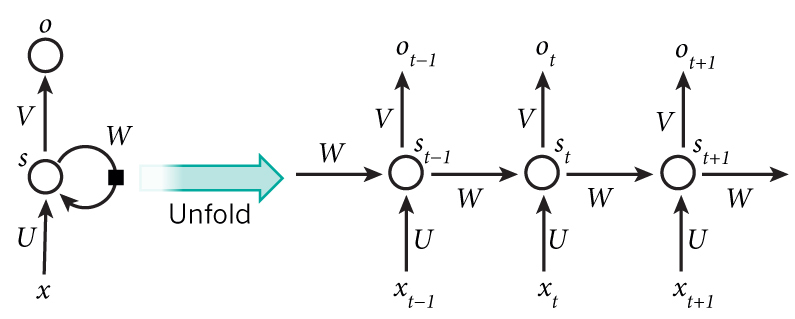
\includegraphics[width=0.8\textwidth]{Rnn2.jpg}
	\caption{循环神经网络}
	\label{fig:Rnn2}
\end{figure}

现在看上去就比较清楚了,这个网络在t时刻接收到输入\({x}_{t}\)之后,隐藏层的值是\({s}_{t}\),输出值是\({o}_{t}\)。关键一点是,\({s}_t\)的值不仅仅取决于\({x}_t\),还取决于\({s}_{t-1}\)。我们可以用下面的公式来表示\textbf{循环神经网络}的计算方法:
\begin{align}
	{o}_t & =g(V{s}_t)\label{eq:Rnn1}            \\
	{s}_t & =f(U{x}_t+W{s}_{t-1})\label{eq:Rnn2}
\end{align}


公式 \ref{eq:Rnn1} 是\textbf{输出层}的计算公式,输出层是一个\textbf{全连接层},也就是它的每个节点都和隐藏层的每个节点相连。$V$是输出层的\textbf{权重矩阵},$g$是\textbf{激活函数}。公式 \ref{eq:Rnn2} 是隐藏层的计算公式,它是\textbf{循环层}。$U$是输入$x$的权重矩阵,$W$是上一次的值\({s}_{t-1}\)作为这一次的输入的\textbf{权重矩阵},$f$是\textbf{激活函数}。

从上面的公式我们可以看出,\textbf{循环层}和\textbf{全连接层}的区别就是\textbf{循环层}多了一个\textbf{权重矩阵}$W$。

如果反复把公式\ref{eq:Rnn2}带入到公式\ref{eq:Rnn1},我们将得到:
\begin{align*}
	{o}_t & =g(V{s}_t)=Vf(U{x}_t+W{s}_{t-1})= g\Big(Vf\big(U{x}_t+Wf(U{x}_{t-1}+W{s}_{t-2})\big)\Big)             \\
	      & = g\Bigg(Vf\Big(U{x}_t+Wf\big(U{x}_{t-1}+Wf(U{x}_{t-2}+W{s}_{t-3})\big)\Big)\Bigg)                    \\
	      & = g\left(Vf\Bigg(U{x}_t+Wf\Big(U{x}_{t-1}+Wf\big(U{x}_{t-2}+Wf(U{x}_{t-3}+...)\big)\Big)\Bigg)\right)
\end{align*}


从上面可以看出,\textbf{循环神经网络}的输出值\(o_t\),是受前面历次输入值\({x}_t\)、\({x}_{t-1}\)、\({x}_{t-2}\)、\({x}_{t-3}\)、...影响的,这就是为什么\textbf{循环神经网络}可以往前看任意多个\textbf{输入值}的原因。




\subsection{双向循环神经网络}\label{Rnn:4}

对于\textbf{语言模型}来说,很多时候光看前面的词是不够的,比如下面这句话:
\begin{lstlisting}[numbers=none]
    我的手机坏了,我打算 _ _ _ _ 一部新手机。
\end{lstlisting}


可以想象,如果我们只看横线前面的词,手机坏了,那么我是打算修一修?换一部新的?还是大哭一场?这些都是无法确定的。但如果我们也看到了横线后面的词是『一部新手机』,那么,横线上的词填『买』的概率就大得多了。

在上一小节中的\textbf{基本循环神经网络}是无法对此进行建模的,因此,我们需要\textbf{双向循环神经网络},如图\ref{fig:Rnn3}所示。

\begin{figure}[!h]
	\centering
	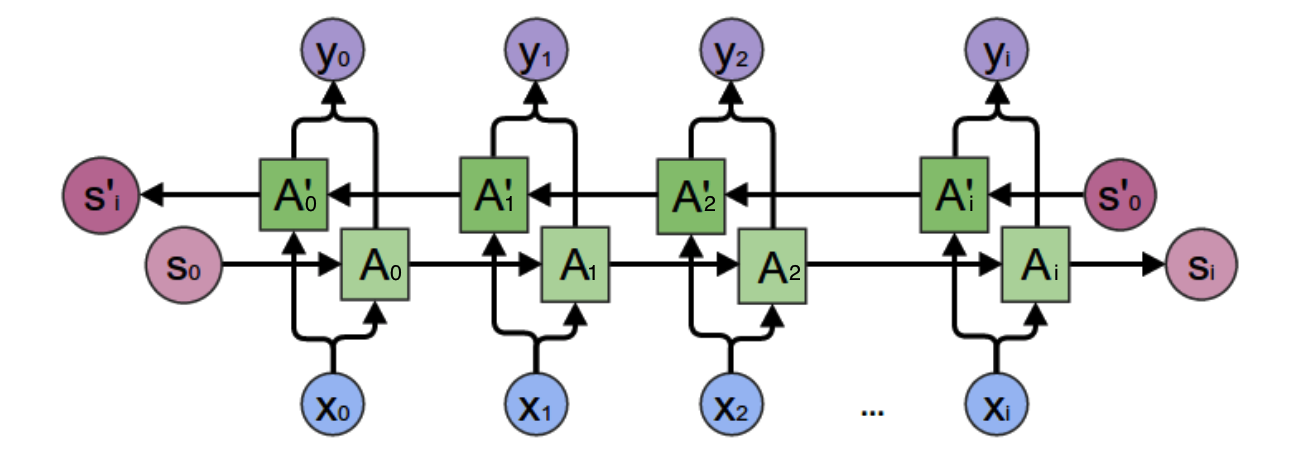
\includegraphics[width=0.8\textwidth]{Rnn3.png}
	\caption{双向循环神经网络}
	\label{fig:Rnn3}
\end{figure}

当遇到这种从未来穿越回来的场景时,难免处于懵逼的状态。不过我们还是可以用屡试不爽的老办法:先分析一个特殊场景,然后再总结一般规律。我们先考虑图\ref{fig:Rnn3}中,\({y}_2\)的计算。

从图\ref{fig:Rnn3}可以看出,\textbf{双向卷积神经网络}的隐藏层要保存两个值,一个$A$参与正向计算,另一个值$A'$参与反向计算。最终的输出值\({y}_2\)取决于\(A_2\)和\(A_2'\)。其计算方法为:
\[
	{y}_2=g(VA_2+V'A_2')
\]

\(A_2\)和\(A_2'\)则分别计算:
\begin{align*}
	A_2  & =f(WA_1+U{x}_2)    \\
	A_2' & =f(W'A_3'+U'{x}_2)
\end{align*}


现在,我们已经可以看出一般的规律:正向计算时,隐藏层的值\({s}_t\)与\({s}_{t-1}\)有关;反向计算时,隐藏层的值\({s}_t'\)与\({s}_{t+1}'\)有关;最终的输出取决于正向和反向计算的\textbf{加和}。现在,我们仿照公式\ref{eq:Rnn1}和\ref{eq:Rnn2},写出双向循环神经网络的计算方法:
\begin{align*}
	{o}_t  & =g(V{s}_t+V'{s}_t')      \\
	{s}_t  & =f(U{x}_t+W{s}_{t-1})    \\
	{s}_t' & =f(U'{x}_t+W'{s}_{t+1}')
\end{align*}


从上面三个公式我们可以看到,正向计算和反向计算\textbf{不共享权重},也就是说$U$和$U'$、$W$和$W'$、$V$和$V'$都是不同的\textbf{权重矩阵}。




\subsection{深度循环神经网络}\label{Rnn:5}
前面我们介绍的\textbf{循环神经网络}只有一个隐藏层,我们当然也可以堆叠两个以上的隐藏层,这样就得到了\textbf{深度循环神经网络}。如图\ref{fig:Rnn4}所示。


我们把第i个隐藏层的值表示为\({s}_t^{(i)}\)、\({s}_t'^{(i)}\),则\textbf{深度循环神经网络}的计算方式可以表示为:
\begin{align*}
	{o}_t        & =g(V^{(i)}{s}_t^{(i)}+V'^{(i)}{s}_t'^{(i)})   \\
	{s}_t^{(i)}  & =f(U^{(i)}{s}_t^{(i-1)}+W^{(i)}{s}_{t-1})     \\
	{s}_t'^{(i)} & =f(U'^{(i)}{s}_t'^{(i-1)}+W'^{(i)}{s}_{t+1}') \\
	...                                                          \\
	{s}_t^{(1)}  & =f(U^{(1)}{x}_t+W^{(1)}{s}_{t-1})             \\
	{s}_t'^{(1)} & =f(U'^{(1)}{x}_t+W'^{(1)}{s}_{t+1}')
\end{align*}


\begin{figure}[!htbp]
	\centering
	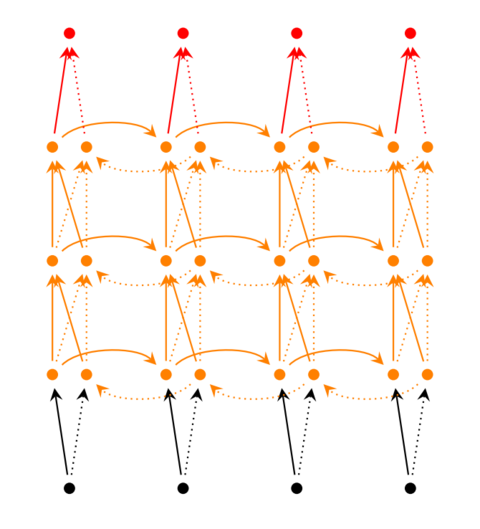
\includegraphics[width=0.4\textwidth]{Rnn4.png}
	\caption{深度循环神经网络}
	\label{fig:Rnn4}
\end{figure}


\section{循环神经网络的训练}\label{Rnn:6}

\subsection{循环神经网络的训练算法:BPTT}\label{Rnn:7}

BPTT算法是针对\textbf{循环层}的训练算法,它的基本原理和BP算法是一样的,也包含同样的三个步骤:

\begin{enumerate}
	\item
	      前向计算每个神经元的输出值;
	\item
	      反向计算每个神经元的\textbf{误差项} \(\delta_j\) 值,它是误差函数$E$对神经元$j$的\textbf{加权输入}\(net_j\)的偏导数;
	\item
	      计算每个权重的梯度。
\end{enumerate}

最后再用\textbf{随机梯度下降}算法更新权重。

循环层如图\ref{fig:Rnn5}所示:

\begin{figure}[!h]
	\centering
	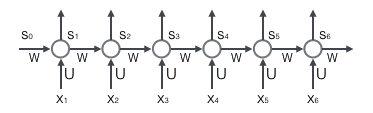
\includegraphics[width=0.6\textwidth]{Rnn5.png}
	\caption{循环层}
	\label{fig:Rnn5}
\end{figure}

\textbf{前向计算}

使用前面的公式\ref{eq:Rnn2}对循环层进行前向计算:
\[
	{s}_t=f(U{x}_t+W{s}_{t-1})
\]

注意,上面的\({s}_t\)、\({x}_t\)、\({s}_{t-1}\)都是向量,用\textbf{黑体字母}表示;而$U$、$V$是\textbf{矩阵},用大写字母表示。\textbf{向量的下标}表示\textbf{时刻},例如,\({s}_t\)表示在$t$时刻向量$s$的值。

我们假设输入向量$x$的维度是$m$,输出向量$s$的维度是$n$,则矩阵$U$的维度是\(n\times m\),矩阵$W$的维度是\(n\times n\)。下面是上式展开成矩阵的样子,看起来更直观一些:
\begin{align*}
	\begin{bmatrix}
		s_1^t  \\
		s_2^t  \\
		\vdots \\
		s_n^t  \\
	\end{bmatrix}=f\left(
	\begin{bmatrix}
		u_{11} u_{12} ... u_{1m} \\
		u_{21} u_{22} ... u_{2m} \\
		\vdots                   \\
		u_{n1} u_{n2} ... u_{nm} \\
	\end{bmatrix}
	\begin{bmatrix}
		x_1^t  \\
		x_2^t  \\
		\vdots \\
		x_m^t  \\
	\end{bmatrix}+
	\begin{bmatrix}
		w_{11} w_{12} ... w_{1n} \\
		w_{21} w_{22} ... w_{2n} \\
		\vdots                   \\
		w_{n1} w_{n2} ... w_{nn} \\
	\end{bmatrix}
	\begin{bmatrix}
		s_1^{t-1} \\
		s_2^{t-1} \\
		\vdots    \\
		s_n^{t-1} \\
	\end{bmatrix}\right)
\end{align*}

在这里我们用\textbf{手写体字母}表示向量的一个\textbf{元素},它的下标表示它是这个向量的第几个元素,它的上标表示第几个\textbf{时刻}。例如,\(s_j^t\)表示向量$s$的第$j$个元素在$t$时刻的值。\(u_{ji}\)表示\textbf{输入层}第$i$个神经元到\textbf{循环层}第$j$个神经元的权重。\(w_{ji}\)表示\textbf{循环层}第$t-1$时刻的第$i$个神经元到\textbf{循环层}第$t$个时刻的第$j$个神经元的权重。

\textbf{误差项的计算}

BTPP算法将第$l$层$t$时刻的\textbf{误差项}\(\delta_t^l\)值沿两个方向传播,一个方向是其传递到上一层网络,得到\(\delta_t^{l-1}\),这部分只和权重矩阵$U$有关;另一个是方向是将其沿时间线传递到初始\(t_1\)时刻,得到\(\delta_1^l\),这部分只和权重矩阵$W$有关。

我们用向量\({net}_t\)表示神经元在$t$时刻的\textbf{加权输入},因为:
\begin{align*}
	{net}_t   & =U{x}_t+W{s}_{t-1} \\
	{s}_{t-1} & =f({net}_{t-1})
\end{align*}


因此:
\begin{align*}
	\frac{\partial{{net}_t}}{\partial{{net}_{t-1}}} & =\frac{\partial{{net}_t}}{\partial{{s}_{t-1}}}\frac{\partial{{s}_{t-1}}}{\partial{{net}_{t-1}}}
\end{align*}


我们用$a$表示列向量,用\({a}^T\)表示行向量。上式的第一项是向量函数对向量求导,其结果为Jacobian矩阵:
\begin{align*}
	\frac{\partial{{net}_t}}{\partial{{s}_{t-1}}} =
	\begin{bmatrix}
		\frac{\partial{net_1^t}}{\partial{s_1^{t-1}}} & \frac{\partial{net_1^t}}{\partial{s_2^{t-1}}} & ... & \frac{\partial{net_1^t}}{\partial{s_n^{t-1}}} \\
		\frac{\partial{net_2^t}}{\partial{s_1^{t-1}}} & \frac{\partial{net_2^t}}{\partial{s_2^{t-1}}} & ... & \frac{\partial{net_2^t}}{\partial{s_n^{t-1}}} \\
		\vdots                                                                                                                                              \\
		\frac{\partial{net_n^t}}{\partial{s_1^{t-1}}} & \frac{\partial{net_n^t}}{\partial{s_2^{t-1}}} & ... & \frac{\partial{net_n^t}}{\partial{s_n^{t-1}}} \\
	\end{bmatrix}
	=\begin{bmatrix}
		w_{11} & w_{12} & ... & w_{1n} \\
		w_{21} & w_{22} & ... & w_{2n} \\
		\vdots                         \\
		w_{n1} & w_{n2} & ... & w_{nn} \\
	\end{bmatrix}=W
\end{align*}


同理,上式第二项也是一个Jacobian矩阵:
\begin{align*}
	\frac{\partial{{s}_{t-1}}}{\partial{{net}_{t-1}}} & =
	\begin{bmatrix}
		\frac{\partial{s_1^{t-1}}}{\partial{net_1^{t-1}}} & \frac{\partial{s_1^{t-1}}}{\partial{net_2^{t-1}}} & ... & \frac{\partial{s_1^{t-1}}}{\partial{net_n^{t-1}}} \\
		\frac{\partial{s_2^{t-1}}}{\partial{net_1^{t-1}}} & \frac{\partial{s_2^{t-1}}}{\partial{net_2^{t-1}}} & ... & \frac{\partial{s_2^{t-1}}}{\partial{net_n^{t-1}}} \\
		\vdots                                                                                                                                                          \\
		\frac{\partial{s_n^{t-1}}}{\partial{net_1^{t-1}}} & \frac{\partial{s_n^{t-1}}}{\partial{net_2^{t-1}}} & ... & \frac{\partial{s_n^{t-1}}}{\partial{net_n^{t-1}}} \\
	\end{bmatrix}                                                      \\
	                                                  & =\begin{bmatrix}
		f'(net_1^{t-1}) & 0               & ... & 0               \\
		0               & f'(net_2^{t-1}) & ... & 0               \\
		\vdots                                                    \\
		0               & 0               & ... & f'(net_n^{t-1}) \\
	\end{bmatrix} \\
	                                                  & =diag[f'({net}_{t-1})]
\end{align*}


其中,$diag({a})$表示根据向量$a$创建一个对角矩阵,即
\[
	diag({a})=\begin{bmatrix}
		a_1 & 0   & ... & 0   \\
		0   & a_2 & ... & 0   \\
		\vdots                \\
		0   & 0   & ... & a_n \\
	\end{bmatrix}
\]

最后,将两项合在一起,可得:
\begin{align*}
	\frac{\partial{{net}_t}}{\partial{{net}_{t-1}}} & =\frac{\partial{{net}_t}}{\partial{{s}_{t-1}}}\frac{\partial{{s}_{t-1}}}{\partial{{net}_{t-1}}}=Wdiag[f'({net}_{t-1})] \\
	                                                & =\begin{bmatrix}
		w_{11}f'(net_1^{t-1}) & w_{12}f'(net_2^{t-1})  & ... & w_{1n}f(net_n^{t-1})   \\
		w_{21}f'(net_1^{t-1}) & w_{22} f'(net_2^{t-1}) & ... & w_{2n}f(net_n^{t-1})   \\
		\vdots                                                                        \\
		w_{n1}f'(net_1^{t-1}) & w_{n2} f'(net_2^{t-1}) & ... & w_{nn} f'(net_n^{t-1}) \\
	\end{bmatrix}
\end{align*}
上式描述了将\(\delta\)沿时间往前传递一个时刻的规律,有了这个规律,我们就可以求得任意时刻$k$的\textbf{误差项}\(\delta_k\):
\begin{align}
	\delta_k^T= & \frac{\partial{E}}{\partial{{net}_k}}=\frac{\partial{E}}{\partial{{net}_t}}\frac{\partial{{net}_t}}{\partial{{net}_k}}=\frac{\partial{E}}{\partial{{net}_t}}\frac{\partial{{net}_t}}{\partial{{net}_{t-1}}}\frac{\partial{{net}_{t-1}}}{\partial{{net}_{t-2}}}...\frac{\partial{{net}_{k+1}}}{\partial{{net}_{k}}}\notag \\
	=           & Wdiag[f'({net}_{t-1})]Wdiag[f'({net}_{t-2})]...Wdiag[f'({net}_{k})]\delta_t^l\notag                                                                                                                                                                                                                                      \\
	=           & \delta_t^T\prod_{i=k}^{t-1}Wdiag[f'({net}_{i})]\label{eq:Rnn3}
\end{align}


公式\ref{eq:Rnn3}就是将误差项沿时间反向传播的算法。

\textbf{循环层}将\textbf{误差项}反向传递到上一层网络,与普通的\textbf{全连接层}是完全一样的,这在第\ref{chap:Bp}章神经网络和反向传播算法中已经详细讲过了,在此仅简要描述一下。

\textbf{循环层}的\textbf{加权输入}\({net}^l\)与上一层的\textbf{加权输入}\({net}^{l-1}\)关系如下:
\begin{align*}
	{net}_t^l=   & U{a}_t^{l-1}+W{s}_{t-1} \\
	{a}_t^{l-1}= & f^{l-1}({net}_t^{l-1})
\end{align*}
上式中\({net}_t^l\)是第$l$层神经元的\textbf{加权输入}(假设第l层是\textbf{循环层});\({net}_t^{l-1}\)是第$l-1$层神经元的\textbf{加权输入};\({a}_t^{l-1}\)是第$l-1$层神经元的输出;\(f^{l-1}\)是第$l-1$层的\textbf{激活函数}。
\[
	\frac{\partial{{net}_t^l}}{\partial{{net}_t^{l-1}}}=\frac{\partial{{net}^l}}{\partial{{a}_t^{l-1}}}\frac{\partial{{a}_t^{l-1}}}{\partial{{net}_t^{l-1}}}=Udiag[f'^{l-1}({net}_t^{l-1})]
\]


所以
\begin{align}
	(\delta_t^{l-1})^T= & \frac{\partial{E}}{\partial{{net}_t^{l-1}}}=\frac{\partial{E}}{\partial{{net}_t^l}}\frac{\partial{{net}_t^l}}{\partial{{net}_t^{l-1}}}\notag \\
	=                   & (\delta_t^l)^TUdiag[f'^{l-1}({net}_t^{l-1})]\label{eq:Rnn4}
\end{align}


公式\ref{eq:Rnn4}就是将误差项传递到上一层算法。

\textbf{权重梯度的计算}

现在,我们终于来到了BPTT算法的最后一步:计算每个权重的梯度。

首先,我们计算误差函数$E$对权重矩阵W的梯度\(\frac{\partial{E}}{\partial{W}}\)。

\begin{figure}[!h]
	\centering
	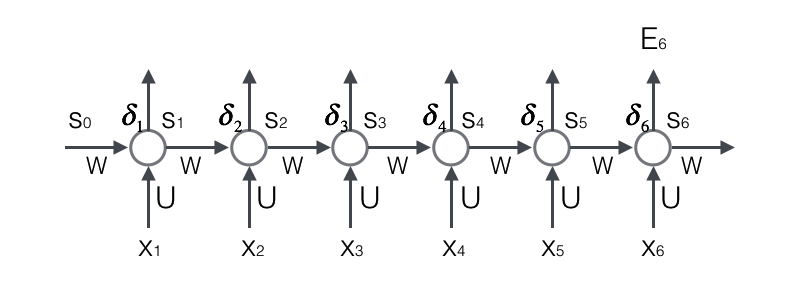
\includegraphics[width=0.8\textwidth]{Rnn6.png}
	\caption{权重梯度}
	\label{fig:Rnn6}
\end{figure}

图\ref{fig:Rnn6}展示了我们到目前为止,在前两步中已经计算得到的量,包括每个时刻t
\textbf{循环层}的输出值\(s_t\),以及误差项\(\delta_t\)。

回忆一下我们在第\ref{chap:Bp}章神经网络和反向传播算法介绍的全连接网络的权重梯度计算算法:只要知道了任意一个时刻的\textbf{误差项}\(\delta_t\),以及上一个时刻循环层的输出值\({s}_{t-1}\),就可以按照下面的公式求出权重矩阵在$t$时刻的梯度\(\nabla_{Wt}E\):
\begin{equation}
	\label{eq:Rnn5}
	\nabla_{W_t}E=\begin{bmatrix}
		\delta_1^ts_1^{t-1} & \delta_1^ts_2^{t-1} & ... & \delta_1^ts_n^{t-1} \\
		\delta_2^ts_1^{t-1} & \delta_2^ts_2^{t-1} & ... & \delta_2^ts_n^{t-1} \\
		\vdots                                                                \\
		\delta_n^ts_1^{t-1} & \delta_n^ts_2^{t-1} & ... & \delta_n^ts_n^{t-1} \\
	\end{bmatrix}
\end{equation}

在公式\ref{eq:Rnn5}中,\(\delta_i^t\)表示t时刻\textbf{误差项}向量的第$i$个分量;\(s_i^{t-1}\)表示$t-1$时刻\textbf{循环层}第$i$个神经元的输出值。

我们下面可以简单推导一下公式\ref{eq:Rnn5}。

我们知道:
\begin{align*}
	{net}_t=                    & U{x}_t+W{s}_{t-1} \\
	\begin{bmatrix}
		net_1^t \\
		net_2^t \\
		\vdots  \\
		net_n^t \\
	\end{bmatrix}= & U{x}_t+
	\begin{bmatrix}
		w_{11} & w_{12} & ... & w_{1n} \\
		w_{21} & w_{22} & ... & w_{2n} \\
		\vdots                         \\
		w_{n1} & w_{n2} & ... & w_{nn} \\
	\end{bmatrix}
	\begin{bmatrix}
		s_1^{t-1} \\
		s_2^{t-1} \\
		\vdots    \\
		s_n^{t-1} \\
	\end{bmatrix}                      \\
	=                           & U{x}_t+
	\begin{bmatrix}
		w_{11}s_1^{t-1}+w_{12}s_2^{t-1} + \cdots + w_{1n}s_n^{t-1} \\
		w_{21}s_1^{t-1}+w_{22}s_2^{t-1} + \cdots + w_{2n}s_n^{t-1} \\
		\vdots                                                     \\
		w_{n1}s_1^{t-1}+w_{n2}s_2^{t-1} + \cdots + w_{nn}s_n^{t-1} \\
	\end{bmatrix}
\end{align*}


因为对$W$求导与\(U{x}_t\)无关,我们不再考虑。现在,我们考虑对权重项\(w_{ji}\)求导。通过观察上式我们可以看到\(w_{ji}\)只与\(net_j^t\)有关,所以:
\[
	\frac{\partial{E}}{\partial{w_{ji}}}=\frac{\partial{E}}{\partial{net_j^t}}\frac{\partial{net_j^t}}{\partial{w_{ji}}}=\delta_j^ts_i^{t-1}
\]


按照上面的规律就可以生成公式\ref{eq:Rnn5}里面的矩阵。

我们已经求得了权重矩阵$W$在$t$时刻的梯度\(\nabla_{Wt}E\),最终的梯度\(\nabla_WE\)是各个时刻的梯度\textbf{之和}:
\begin{align}
	\nabla_WE= & \sum_{i=1}^t\nabla_{W_i}E\notag \\
	=          & \begin{bmatrix}
		\delta_1^ts_1^{t-1} & \delta_1^ts_2^{t-1} & ... & \delta_1^ts_n^{t-1} \\
		\delta_2^ts_1^{t-1} & \delta_2^ts_2^{t-1} & ... & \delta_2^ts_n^{t-1} \\
		\vdots                                                                \\
		\delta_n^ts_1^{t-1} & \delta_n^ts_2^{t-1} & ... & \delta_n^ts_n^{t-1} \\
	\end{bmatrix}+...+
	\begin{bmatrix}
		\delta_1^1s_1^0 & \delta_1^1s_2^0 & ... & \delta_1^1s_n^0 \\
		\delta_2^1s_1^0 & \delta_2^1s_2^0 & ... & \delta_2^1s_n^0 \\
		\vdots                                                    \\
		\delta_n^1s_1^0 & \delta_n^1s_2^0 & ... & \delta_n^1s_n^0 \\
	\end{bmatrix}\label{eq:Rnn6}
\end{align}

公式\ref{eq:Rnn6}就是计算\textbf{循环层}权重矩阵$W$的梯度的公式。

\textbf{——数学公式超高能预警——}

前面已经介绍了\(\nabla_WE\)的计算方法,看上去还是比较直观的。然而,读者也许会困惑,为什么最终的梯度是各个时刻的梯度\textbf{之和}呢?我们前面只是直接用了这个结论,实际上这里面是有道理的,只是这个数学推导比较绕脑子。感兴趣的同学可以仔细阅读接下来这一段,它用到了矩阵对矩阵求导、张量与向量相乘运算的一些法则。

我们还是从这个式子开始:
\[
	{net}_t=U{x}_t+Wf({net}_{t-1})
\]

因为\(U{x}_t\)与$W$完全无关,我们把它看做常量。现在,考虑第一个式子加号右边的部分,因为$W$和\(f({net}_{t-1})\)都是$W$的函数,因此我们要用到大学里面都学过的导数乘法运算:
\[
	(uv)'=u'v+uv'
\]

因此,上面第一个式子写成:
\[
	\frac{\partial{{net}_t}}{\partial{W}}=\frac{\partial{W}}{\partial{W}}f({net}_{t-1})+W\frac{\partial{f({net}_{t-1})}}{\partial{W}}\\
\]

我们最终需要计算的是\(\nabla_WE\):
\begin{align}
	\nabla_WE= & \frac{\partial{E}}{\partial{W}}=\frac{\partial{E}}{\partial{{net}_t}}\frac{\partial{{net}_t}}{\partial{W}}\notag                \\
	=          & \delta_t^T\frac{\partial{W}}{\partial{W}}f({net}_{t-1})+ \delta_t^TW\frac{\partial{f({net}_{t-1})}}{\partial{W}}\label{eq:Rnn7}
\end{align}

我们先计算公式\ref{eq:Rnn7}加号左边的部分。\(\frac{\partial{W}}{\partial{W}}\)是\textbf{矩阵对矩阵求导},其结果是一个四维\textbf{张量(tensor)},如下所示:

\begin{align*}
	\frac{\partial{W}}{\partial{W}}= &
	\begin{bmatrix}
		\frac{\partial{w_{11}}}{\partial{W}} & \frac{\partial{w_{12}}}{\partial{W}} & ... & \frac{\partial{w_{1n}}}{\partial{W}} \\
		\frac{\partial{w_{21}}}{\partial{W}} & \frac{\partial{w_{22}}}{\partial{W}} & ... & \frac{\partial{w_{2n}}}{\partial{W}} \\\vdots \\
		\frac{\partial{w_{n1}}}{\partial{W}} & \frac{\partial{w_{n2}}}{\partial{W}} & ... & \frac{\partial{w_{nn}}}{\partial{W}} \\
	\end{bmatrix}         \\
	=                                &
	\begin{bmatrix}
		\begin{bmatrix}
			\frac{\partial{w_{11}}}{\partial{w_{11}}} & \frac{\partial{w_{11}}}{\partial{w_{12}}} & ... & \frac{\partial{w_{11}}}{\partial{_{1n}}} \\
			\frac{\partial{w_{11}}}{\partial{w_{21}}} & \frac{\partial{w_{11}}}{\partial{w_{22}}} & ... & \frac{\partial{w_{11}}}{\partial{_{2n}}} \\\vdots\\
			\frac{\partial{w_{11}}}{\partial{w_{n1}}} & \frac{\partial{w_{11}}}{\partial{w_{n2}}} & ... & \frac{\partial{w_{11}}}{\partial{_{nn}}} \\
		\end{bmatrix} &
		\begin{bmatrix}
			\frac{\partial{w_{12}}}{\partial{w_{11}}} & \frac{\partial{w_{12}}}{\partial{w_{12}}} & ... & \frac{\partial{w_{12}}}{\partial{_{1n}}} \\
			\frac{\partial{w_{12}}}{\partial{w_{21}}} & \frac{\partial{w_{12}}}{\partial{w_{22}}} & ... & \frac{\partial{w_{12}}}{\partial{_{2n}}} \\\vdots\\
			\frac{\partial{w_{12}}}{\partial{w_{n1}}} & \frac{\partial{w_{12}}}{\partial{w_{n2}}} & ... & \frac{\partial{w_{12}}}{\partial{_{nn}}} \\
		\end{bmatrix} & ... \\\vdots\\
	\end{bmatrix}         \\
	=                                &
	\begin{bmatrix}
		\begin{bmatrix}
			1 & 0 & ... & 0 \\
			0 & 0 & ... & 0 \\
			\vdots          \\
			0 & 0 & ... & 0 \\
		\end{bmatrix} &
		\begin{bmatrix}
			0 & 1 & ... & 0 \\
			0 & 0 & ... & 0 \\
			\vdots          \\
			0 & 0 & ... & 0 \\
		\end{bmatrix} & ... \\
		\vdots                           \\
	\end{bmatrix}
\end{align*}


接下来,我们知道\(s_{t-1}=f({{net}_{t-1}})\),它是一个\textbf{列向量}。我们让上面的四维张量与这个向量相乘,得到了一个三维张量,再左乘行向量\(\delta_t^T\),最终得到一个矩阵:

\begin{align*}
	\delta_t^T\frac{\partial{W}}{\partial{W}}f({{net}_{t-1}})= & \delta_t^T\frac{\partial{W}}{\partial{W}}{{s}_{t-1}}=\delta_t^T
	\begin{bmatrix}
		\begin{bmatrix}
			1 & 0 & ... & 0 \\
			0 & 0 & ... & 0 \\
			\vdots          \\
			0 & 0 & ... & 0 \\
		\end{bmatrix} &
		\begin{bmatrix}
			0 & 1 & ... & 0 \\
			0 & 0 & ... & 0 \\
			\vdots          \\
			0 & 0 & ... & 0 \\
		\end{bmatrix} & ... \\
		\vdots                           \\
	\end{bmatrix}
	\begin{bmatrix}
		s_1^{t-1} \\
		s_2^{t-1} \\
		\vdots    \\
		s_n^{t-1} \\
	\end{bmatrix}                                                                                                   \\
	=                                                          & \delta_t^T
	\begin{bmatrix}
		\begin{bmatrix}
			s_1^{t-1} \\
			0         \\
			\vdots    \\
			0         \\
		\end{bmatrix} &
		\begin{bmatrix}
			s_2^{t-1} \\
			0         \\
			\vdots    \\
			0         \\
		\end{bmatrix} & ... \\
		\vdots                           \\
	\end{bmatrix}=
	\begin{bmatrix}
		\delta_1^t & \delta_2^t & ... & \delta_n^t
	\end{bmatrix}
	\begin{bmatrix}
		\begin{bmatrix}
			s_1^{t-1} \\
			0         \\
			\vdots    \\
			0         \\
		\end{bmatrix} &
		\begin{bmatrix}
			s_2^{t-1} \\
			0         \\
			\vdots    \\
			0         \\
		\end{bmatrix} & ... \\
		\vdots                           \\
	\end{bmatrix}                                                                                                   \\
	=                                                          &
	\begin{bmatrix}
		\delta_1^ts_1^{t-1} & \delta_1^ts_2^{t-1} & ... & \delta_1^ts_n^{t-1} \\
		\delta_2^ts_1^{t-1} & \delta_2^ts_2^{t-1} & ... & \delta_2^ts_n^{t-1} \\
		\vdots                                                                \\
		\delta_n^ts_1^{t-1} & \delta_n^ts_2^{t-1} & ... & \delta_n^ts_n^{t-1} \\
	\end{bmatrix}=\nabla_{Wt}E
\end{align*}


接下来,我们计算公式\ref{eq:Rnn7}加号右边的部分:
\begin{align*}
	\delta_t^TW\frac{\partial{f({net}_{t-1})}}{\partial{W}}= & \delta_t^TW\frac{\partial{f({net}_{t-1})}}{\partial{{net}_{t-1}}}\frac{\partial{{net}_{t-1}}}{\partial{W}}=\delta_t^TWf'({net}_{t-1})\frac{\partial{{net}_{t-1}}}{\partial{W}} \\
	=                                                        & \delta_t^T\frac{\partial{{net}_t}}{\partial{{net}_{t-1}}}\frac{\partial{{net}_{t-1}}}{\partial{W}}=\delta_{t-1}^T\frac{\partial{{net}_{t-1}}}{\partial{W}}
\end{align*}


于是,我们得到了如下递推公式:
\begin{align*}
	\nabla_WE= & \frac{\partial{E}}{\partial{W}}=\frac{\partial{E}}{\partial{{net}_t}}\frac{\partial{{net}_t}}{\partial{W}}=\nabla_{Wt}E+\delta_{t-1}^T\frac{\partial{{net}_{t-1}}}{\partial{W}} \\
	=          & \nabla_{Wt}E+\nabla_{Wt-1}E+\delta_{t-2}^T\frac{\partial{{net}_{t-2}}}{\partial{W}}                                                                                             \\
	=          & \nabla_{Wt}E+\nabla_{Wt-1}E+...+\nabla_{W1}E                                                                                                                                    \\
	=          & \sum_{k=1}^t\nabla_{Wk}E
\end{align*}

这样,我们就证明了:最终的梯度\(\nabla_WE\)是各个时刻的梯度之和。

\textbf{---数学公式超高能预警解除---}

同权重矩阵$W$类似,我们可以得到权重矩阵$U$的计算方法。

\begin{equation}
	\label{eq:Rnn8}
	\nabla_{U_t}E=\begin{bmatrix}
		\delta_1^tx_1^t & \delta_1^tx_2^t & ... & \delta_1^tx_m^t \\
		\delta_2^tx_1^t & \delta_2^tx_2^t & ... & \delta_2^tx_m^t \\
		\vdots                                                    \\
		\delta_n^tx_1^t & \delta_n^tx_2^t & ... & \delta_n^tx_m^t \\
	\end{bmatrix}
\end{equation}

公式\ref{eq:Rnn8}是误差函数在$t$时刻对权重矩阵$U$的梯度。和权重矩阵$W$一样,最终的梯度也是各个时刻的梯度之和:
\[
	\nabla_UE=\sum_{i=1}^t\nabla_{U_i}E
\]

具体的证明这里就不再赘述了,感兴趣的读者可以练习推导一下。

\subsection{RNN的梯度爆炸和消失问题}\label{Rnn:8}

不幸的是,实践中前面介绍的几种RNNs并不能很好的处理较长的序列。一个主要的原因是,RNN在训练中很容易发生\textbf{梯度爆炸}和\textbf{梯度消失},这导致训练时梯度不能在较长序列中一直传递下去,从而使RNN无法捕捉到长距离的影响。

为什么RNN会产生梯度爆炸和消失问题呢?我们接下来将详细分析一下原因。我们根据公式\ref{eq:Rnn3}可得:
\begin{align*}
	\delta_k^T=             & \delta_t^T\prod_{i=k}^{t-1}Wdiag[f'(\mathrm{net}_{i})]             \\
	\|\delta_k^T\|\leqslant & \|\delta_t^T\|\prod_{i=k}^{t-1}\|W\|\|diag[f'(\mathrm{net}_{i})]\| \\
	\leqslant               & \|\delta_t^T\|(\beta_W\beta_f)^{t-k}
\end{align*}

上式的\(\beta\)定义为矩阵的模的上界。因为上式是一个指数函数,如果$t-k$很大的话(也就是向前看很远的时候),会导致对应的\textbf{误差项}的值增长或缩小的非常快,这样就会导致相应的\textbf{梯度爆炸}和\textbf{梯度消失}问题(取决于\(\beta\)大于1还是小于1)。

通常来说,\textbf{梯度爆炸}更容易处理一些。因为梯度爆炸的时候,我们的程序会收到$NaN$错误。我们也可以设置一个梯度阈值,当梯度超过这个阈值的时候可以直接截取。

\textbf{梯度消失}更难检测,而且也更难处理一些。总的来说,我们有三种方法应对梯度消失问题:

\begin{enumerate}
	\item
	      合理的初始化权重值。初始化权重,使每个神经元尽可能不要取极大或极小值,以躲开梯度消失的区域。
	\item
	      使用relu代替sigmoid和tanh作为激活函数。原理请参考第\ref{chap:Cnn}章卷积神经网络的\ref{Cnn:1}\textbf{激活函数}一节。
	\item
	      使用其他结构的RNNs,比如长短时记忆网络(LTSM)和Gated Recurrent   Unit(GRU),这是最流行的做法。我们将在以后的文章中介绍这两种网络。
\end{enumerate}







\section{RNN的应用:基于RNN的语言模型}\label{Rnn:9}

现在,我们介绍一下基于RNN语言模型。我们首先把词依次输入到循环神经网络中,每输入一个词,循环神经网络就输出截止到目前为止,下一个最可能的词。例如,当我们依次输入:
\begin{lstlisting}[numbers=none]
    我 昨天 上学 迟到 了
\end{lstlisting}

神经网络的输出如图\ref{fig:Rnn7}所示:
\begin{figure}[!h]
	\centering
	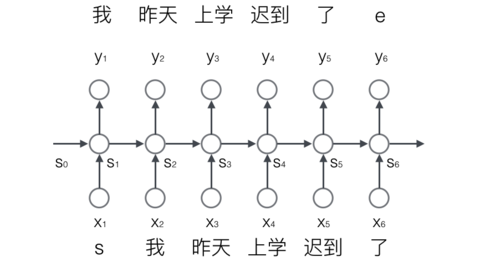
\includegraphics[width=0.7\textwidth]{Rnn7.png}
	\caption{神经网络的输出}
	\label{fig:Rnn7}
\end{figure}

其中,s和e是两个特殊的词,分别表示一个序列的开始和结束。

\subsection{向量化}\label{Rnn:10}

我们知道,神经网络的输入和输出都是\textbf{向量},为了让语言模型能够被神经网络处理,我们必须把词表达为向量的形式,这样神经网络才能处理它。

神经网络的输入是\textbf{词},我们可以用下面的步骤对输入进行\textbf{向量化}:

\begin{enumerate}
	\item
	      建立一个包含所有词的词典,每个词在词典里面有一个唯一的编号。
	\item
	      任意一个词都可以用一个$N$维的one-hot向量来表示。其中,$N$是词典中包含的词的个数。假设一个词在词典中的编号是$i$,$v$是表示这个词的向量,\(v_j\)是向量的第$j$个元素,则:
	      \begin{equation*}
		      v_j=\left\{
		      \begin{aligned}
			      1 & \quad j=i       \\
			      0 & \quad otherwise
		      \end{aligned}
		      \right.
	      \end{equation*}
\end{enumerate}


上面这个公式的含义,可以用图\ref{fig:Rnn8}来直观的表示。
\begin{figure}[!h]
	\centering
	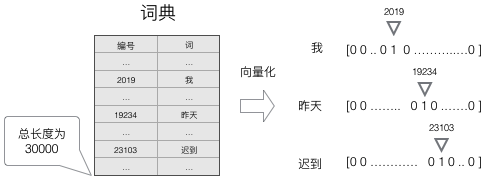
\includegraphics[width=0.9\textwidth]{Rnn8.png}
	\caption{向量化}
	\label{fig:Rnn8}
\end{figure}
使用这种向量化方法,我们就得到了一个高维、\textbf{稀疏}的向量(稀疏是指绝大部分元素的值都是0)。处理这样的向量会导致我们的神经网络有很多的参数,带来庞大的计算量。因此,往往会需要使用一些降维方法,将高维的稀疏向量转变为低维的稠密向量。不过这个话题我们就不再这篇文章中讨论了。

语言模型要求的输出是下一个最可能的词,我们可以让循环神经网络计算计算词典中每个词是下一个词的概率,这样,概率最大的词就是下一个最可能的词。因此,神经网络的输出向量也是一个$N$维向量,向量中的每个元素对应着词典中相应的词是下一个词的概率。如图\ref{fig:Rnn9}所示:

\begin{figure}[!h]
	\centering
	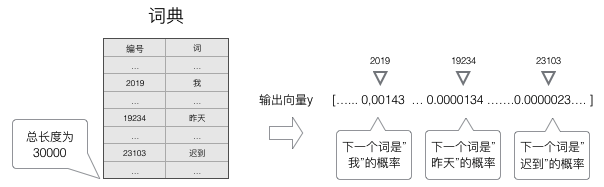
\includegraphics[width=0.9\textwidth]{Rnn9.png}
	\caption{向量化}
	\label{fig:Rnn9}
\end{figure}

\subsection{Softmax层}\label{Rnn:11}

前面提到,\textbf{语言模型}是对下一个词出现的\textbf{概率}进行建模。那么,怎样让神经网络输出概率呢?方法就是用softmax层作为神经网络的输出层。

我们先来看一下softmax函数的定义:
\[
	g(z_i)=\frac{e^{z_i}}{\sum_{k}e^{z_k}}
\]

这个公式看起来可能很晕,我们举一个例子。Softmax层如图\ref{fig:Rnn10}所示,
从图\ref{fig:Rnn10}我们可以看到,softmax layer的输入是一个向量,输出也是一个向量,两个向量的维度是一样的(在这个例子里面是4)。输入向量$x=[1, 2, 3, 4]$经过softmax层之后,经过上面的softmax函数计算,转变为输出向量$y=[0.03, 0.09, 0.24, 0.64]$。计算过程为:
\begin{align*}
	y_1 & =\frac{e^{x_1}}{\sum_{k}e^{x_k}}=\frac{e^1}{e^1+e^2+e^3+e^4}=0.03 \\
	y_2 & =\frac{e^2}{e^1+e^2+e^3+e^4}=0.09                                 \\
	y_3 & =\frac{e^3}{e^1+e^2+e^3+e^4}=0.24                                 \\
	y_4 & =\frac{e^4}{e^1+e^2+e^3+e^4}=0.64
\end{align*}

\begin{figure}[!h]
	\centering
	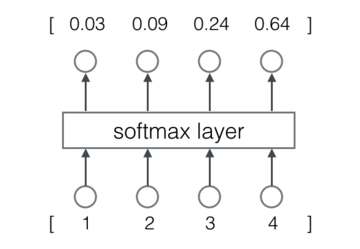
\includegraphics[width=0.5\textwidth]{Rnn10.png}
	\caption{Softmax层}
	\label{fig:Rnn10}
\end{figure}

我们来看看输出向量$y$的特征:

\begin{enumerate}
	\item
	      每一项为取值为0-1之间的正数;
	\item
	      所有项的总和是1。
\end{enumerate}

我们不难发现,这些特征和\textbf{概率}的特征是一样的,因此我们可以把它们看做是概率。对于\textbf{语言模型}来说,我们可以认为模型预测下一个词是词典中第一个词的概率是0.03,是词典中第二个词的概率是0.09,以此类推。

\subsection{语言模型的训练}\label{Rnn:12}

可以使用\textbf{监督学习}的方法对语言模型进行训练,首先,需要准备训练数据集。接下来,我们介绍怎样把语料
\begin{lstlisting}[numbers=none]
    我 昨天 上学 迟到 了
\end{lstlisting}

转换成语言模型的训练数据集。

首先,我们获取\textbf{输入-标签}对:

\begin{table}[!h]
	\centering
	\setlength{\tabcolsep}{10mm}
	\caption{输入-标签}
	\begin{tabular}{cc}
		\hline
		输入 & 标签 \\ \hline
		s    & 我   \\
		我   & 昨天 \\
		昨天 & 上学 \\
		上学 & 迟到 \\
		迟到 & 了   \\
		了   & e    \\ \hline
	\end{tabular}
\end{table}


然后,使用前面介绍过的\textbf{向量化}方法,对输入$x$和标签$y$进行\textbf{向量化}。这里面有意思的是,对标签$y$进行向量化,其结果也是一个one-hot向量。例如,我们对标签『我』进行向量化,得到的向量中,只有第2019个元素的值是1,其他位置的元素的值都是0。它的含义就是下一个词是『我』的概率是1,是其它词的概率都是0。

最后,我们使用\textbf{交叉熵误差函数}作为优化目标,对模型进行优化。

在实际工程中,我们可以使用大量的语料来对模型进行训练,获取训练数据和训练的方法都是相同的。

\subsection{交叉熵误差}\label{Rnn:13}

一般来说,当神经网络的输出层是softmax层时,对应的误差函数$S$通常选择交叉熵误差函数,其定义如下:
\[
	L(y,o)=-\frac{1}{N}\sum_{n\in{N}}{y_nlogo_n}
\]

在上式中,$N$是训练样本的个数,向量\(y_n\)是样本的标记,向量\(o_n\)是网络的输出。标记\(y_n\)是一个one-hot向量,例如\(y_1=[1,0,0,0]\),如果网络的输出\(o=[0.03,0.09,0.24,0.64]\),那么,交叉熵误差是(假设只有一个训练样本,即N=1):
\begin{align*}
	L & =-\frac{1}{N}\sum_{n\in{N}}{y_nlogo_n}=-y_1logo_1 \\
	  & =-(1*log0.03+0*log0.09+0*log0.24+0*log0.64)=3.51
\end{align*}


我们当然可以选择其他函数作为我们的误差函数,比如最小平方误差函数(MSE)。不过对概率进行建模时,选择交叉熵误差函数更make sense。具体原因,感兴趣的读者请阅读(\url{https://jamesmccaffrey.wordpress.com/2011/12/17/neural-network-classification-categorical-data-softmax-activation-and-cross-entropy-error/})。




\section{编程实战:RNN的实现}\label{Rnn:14}

\begin{note}
	完整代码请参考GitHub: \url{https://github.com/hanbt/learn_dl/blob/master/rnn.py}
	(python2.7)
\end{note}

为了加深我们对前面介绍的知识的理解,我们来动手实现一个RNN层。我们复用了第\ref{chap:Cnn}章卷积神经网络中的一些代码,所以先把它们导入进来。
\begin{lstlisting}
import numpy as np
from cnn import ReluActivator, IdentityActivator, element_wise_op
\end{lstlisting}

我们用RecurrentLayer类来实现一个\textbf{循环层}。下面的代码是初始化一个循环层,可以在构造函数中设置卷积层的超参数。我们注意到,循环层有两个权重数组,U和W。
\begin{lstlisting}
class RecurrentLayer(object):
    def __init__(self, input_width, state_width,
                 activator, learning_rate):
        self.input_width = input_width
        self.state_width = state_width
        self.activator = activator
        self.learning_rate = learning_rate
        self.times = 0       # 当前时刻初始化为t0
        self.state_list = [] # 保存各个时刻的state
        self.state_list.append(np.zeros(
            (state_width, 1)))           # 初始化s0
        self.U = np.random.uniform(-1e-4, 1e-4,
            (state_width, input_width))  # 初始化U
        self.W = np.random.uniform(-1e-4, 1e-4,
            (state_width, state_width))  # 初始化W
\end{lstlisting}

在forward方法中,实现循环层的前向计算,这部分比较简单。
\begin{lstlisting}
    def forward(self, input_array):
        '''
        根据『式2』进行前向计算
        '''
        self.times += 1
        state = (np.dot(self.U, input_array) +
                 np.dot(self.W, self.state_list[-1]))
        element_wise_op(state, self.activator.forward)
        self.state_list.append(state)
\end{lstlisting}

在backword方法中,实现BPTT算法。
\begin{lstlisting}
    def backward(self, sensitivity_array, 
                 activator):
        '''
        实现BPTT算法
        '''
        self.calc_delta(sensitivity_array, activator)
        self.calc_gradient()
    def calc_delta(self, sensitivity_array, activator):
        self.delta_list = []  # 用来保存各个时刻的误差项
        for i in range(self.times):
            self.delta_list.append(np.zeros(
                (self.state_width, 1)))
        self.delta_list.append(sensitivity_array)
        # 迭代计算每个时刻的误差项
        for k in range(self.times - 1, 0, -1):
            self.calc_delta_k(k, activator)
    def calc_delta_k(self, k, activator):
        '''
        根据k+1时刻的delta计算k时刻的delta
        '''
        state = self.state_list[k+1].copy()
        element_wise_op(self.state_list[k+1],
                    activator.backward)
        self.delta_list[k] = np.dot(
            np.dot(self.delta_list[k+1].T, self.W),
            np.diag(state[:,0])).T
    def calc_gradient(self):
        self.gradient_list = [] # 保存各个时刻的权重梯度
        for t in range(self.times + 1):
            self.gradient_list.append(np.zeros(
                (self.state_width, self.state_width)))
        for t in range(self.times, 0, -1):
            self.calc_gradient_t(t)
        # 实际的梯度是各个时刻梯度之和
        self.gradient = reduce(
            lambda a, b: a + b, self.gradient_list,
            self.gradient_list[0]) # [0]被初始化为0且没有被修改过
    def calc_gradient_t(self, t):
        '''
        计算每个时刻t权重的梯度
        '''
        gradient = np.dot(self.delta_list[t],
            self.state_list[t-1].T)
        self.gradient_list[t] = gradient
\end{lstlisting}

有意思的是,BPTT算法虽然数学推导的过程很麻烦,但是写成代码却并不复杂。

在update方法中,实现梯度下降算法。
\begin{lstlisting}
    def update(self):
        '''
        按照梯度下降,更新权重
        '''
        self.W -= self.learning_rate * self.gradient
\end{lstlisting}

上面的代码不包含权重U的更新。这部分实际上和全连接神经网络是一样的,留给感兴趣的读者自己来完成吧。

\textbf{循环层}是一个\textbf{带状态}的层,每次forword都会改变循环层的内部状态,这给梯度检查带来了麻烦。因此,我们需要一个reset\_state方法,来重置循环层的内部状态。
\begin{lstlisting}
    def reset_state(self):
        self.times = 0       # 当前时刻初始化为t0
        self.state_list = [] # 保存各个时刻的state
        self.state_list.append(np.zeros(
            (self.state_width, 1)))      # 初始化s0
\end{lstlisting}

最后,是梯度检查的代码。
\begin{lstlisting}
def gradient_check():
    '''
    梯度检查
    '''
    # 设计一个误差函数,取所有节点输出项之和
    error_function = lambda o: o.sum()
    rl = RecurrentLayer(3, 2, IdentityActivator(), 1e-3)
    # 计算forward值
    x, d = data_set()
    rl.forward(x[0])
    rl.forward(x[1])
    # 求取sensitivity map
    sensitivity_array = np.ones(rl.state_list[-1].shape,
                                dtype=np.float64)
    # 计算梯度
    rl.backward(sensitivity_array, IdentityActivator())
    # 检查梯度
    epsilon = 10e-4
    for i in range(rl.W.shape[0]):
        for j in range(rl.W.shape[1]):
            rl.W[i,j] += epsilon
            rl.reset_state()
            rl.forward(x[0])
            rl.forward(x[1])
            err1 = error_function(rl.state_list[-1])
            rl.W[i,j] -= 2*epsilon
            rl.reset_state()
            rl.forward(x[0])
            rl.forward(x[1])
            err2 = error_function(rl.state_list[-1])
            expect_grad = (err1 - err2) / (2 * epsilon)
            rl.W[i,j] += epsilon
            print 'weights(%d,%d): expected - actural %f - %f' % (
                i, j, expect_grad, rl.gradient[i,j])
\end{lstlisting}

需要注意,每次计算error之前,都要调用reset\_state方法重置循环层的内部状态。下面是梯度检查的结果,没问题!

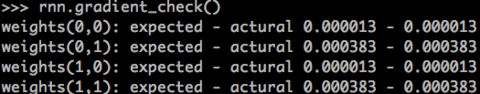
\includegraphics[width=0.7\textwidth]{Rnn11.png}


\section{小节}

至此,我们讲完了基本的\textbf{循环神经网络}、它的训练算法:\textbf{BPTT},以及在语言模型上的应用。RNN比较烧脑,相信拿下前几篇文章的读者们搞定这篇文章也不在话下吧!然而,\textbf{循环神经网络}这个话题并没有完结。我们在前面说到过,基本的循环神经网络存在梯度爆炸和梯度消失问题,并不能真正的处理好长距离的依赖(虽然有一些技巧可以减轻这些问题)。事实上,真正得到广泛的应用的是循环神经网络的一个变体:\textbf{长短时记忆网络}。它内部有一些特殊的结构,可以很好的处理长距离的依赖,我们将在下一篇文章中详细的介绍它。现在,让我们稍事休息,准备挑战更为烧脑的\textbf{长短时记忆网络}吧。


